\subsection{Cloud Computing}

Cloud computing is a form of distributed computing that turns compute infrastructure, programming
platforms and software systems into scalable utility services. By exposing various compute and programming
resources as utility services, cloud computing promotes resource sharing at scale via the Internet.
Depending on the type of resources
offered as services, cloud computing platforms can be categorized into three main categories:

\begin{description}
\item [Infrastructure-as-a-Service clouds (IaaS)]
Offers low-level compute, storage and networking
resources as a service. Compute resources are typically provided in the form of on-demand virtual machines 
with specific CPU, memory and disk configurations (e.g. Amazon EC2, Google Compute Engine, Eucalyptus). 
\item [Platform-as-a-Service clouds (PaaS)]
Offers a programming platform as a service, that can be used to develop and deploy applications at scale 
(e.g. Google App Engine, Heroku, Amazon Elastic Beanstalk).
\item [Software-as-a-Service clouds (SaaS)]
Offers a collection of software applications and tools as a service, that can be directly consumed by
application endusers (e.g. Salesforce, Workday, Citrix go2meeting). This can be thought of as a new way 
of delivering software to
endusers. Instead of prompting the users to download and install any software, SaaS enables the users
to consume software via the Internet.  
\end{description}

Due to the benefits associated with cloud computing (scalability, high availability, productivity enhancement etc.),
many developers and organizations have adopted the cloud as their preferred means of developing, deploying and
delivering software applications. Such cloud-hosted applications expose one or more web application programming 
interfaces (web APIs) through which users can remotely interact with the applications. A cloud-hosted 
application may
also consume web APIs exposed by other cloud-hosted applications. Thus, cloud-hosted applications
form an intricate graph of inter-dependencies among them, where each application can service a set of
applications, while being dependent on a set of other applications. However, in general, each cloud-hosted
application directly depends on the core services offered by the underlying cloud platform for compute power, storage,
network connectivity and scalability.

In the next subsection we take a closer look at a specific type of cloud platforms -- Platform-as-a-Service clouds.
We use PaaS clouds as a case study and a testbed in a number of our explorations.

\subsection{Platform-as-a-Service Clouds}
PaaS clouds provide a managed application programming platform, where an application developer can simply 
write some code, and run it at scale at the push of a button. It relieves the developer from having to install or configure
any hardware resources, virtual machines or operating systems. Everything an application requires is provisioned
and managed by the PaaS cloud. PaaS clouds are specifically built for deploying and running applications -- 
applications that are directly consumed by end users and other client applications. This means, all the problems 
outlined earlier, such as poor development practices, performance SLAs and performance debugging directly 
impact PaaS clouds. 

\begin{figure}
\centering
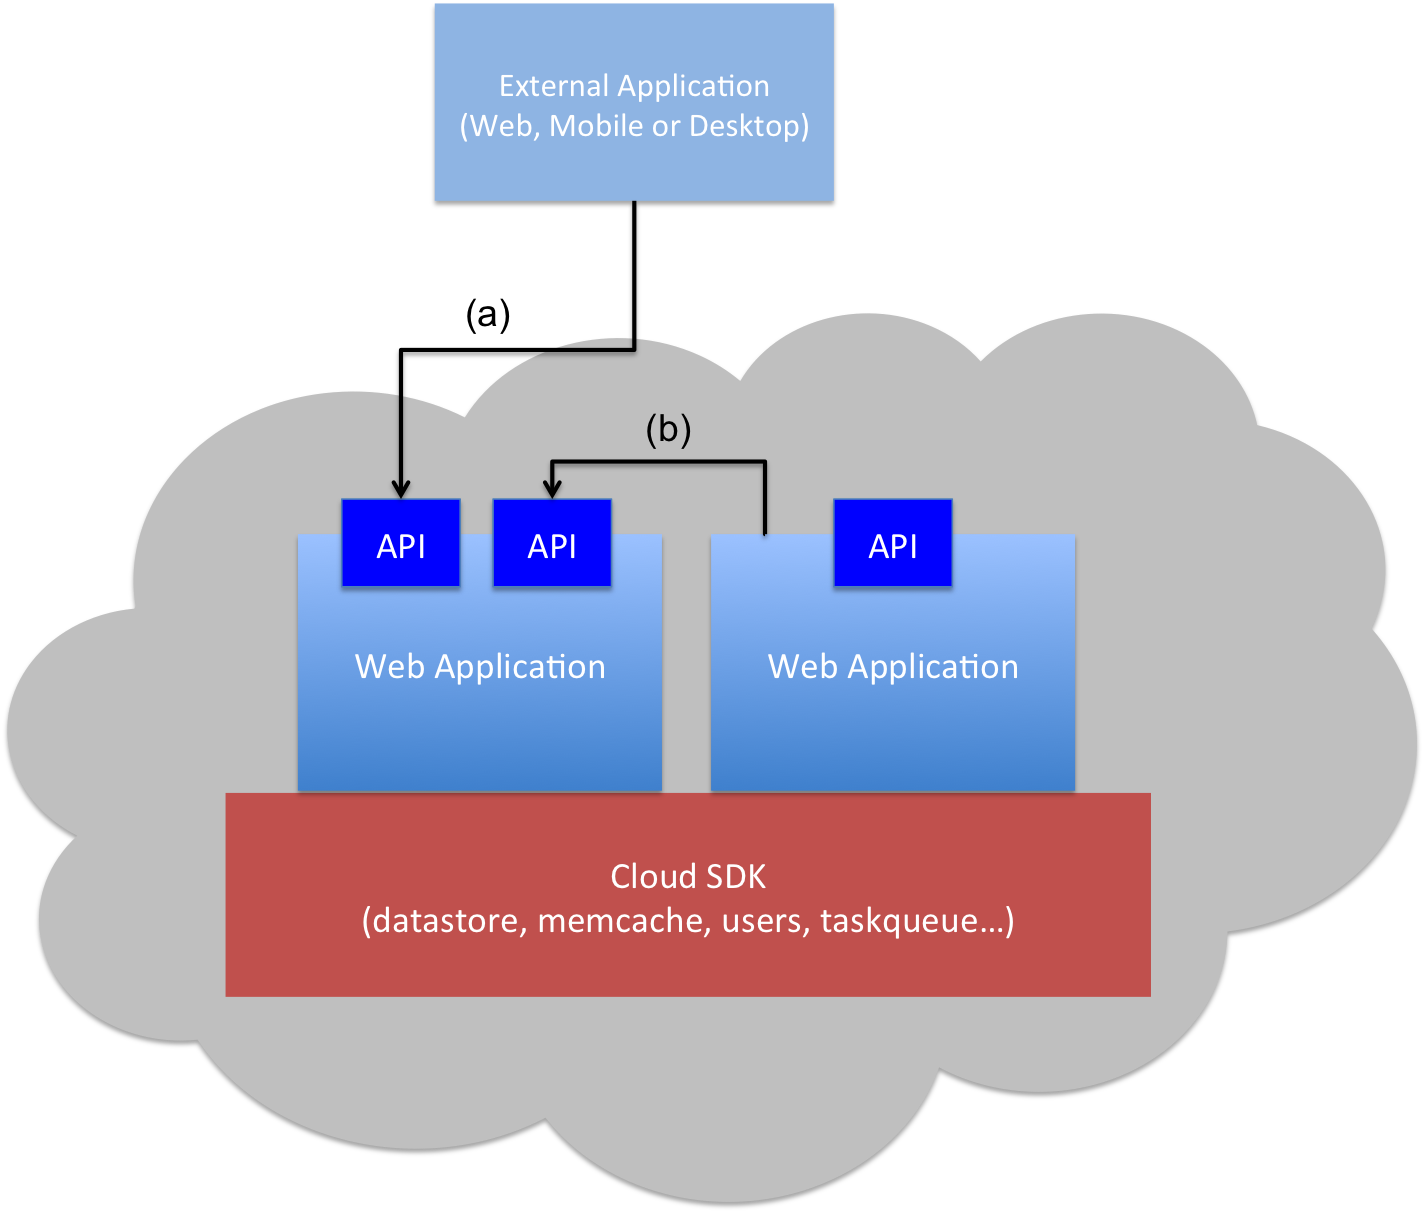
\includegraphics[scale=0.35]{cloud_app_model}
\caption{Applications deployed in a PaaS cloud: (a) An external client making requests
to an application via the web API;
(b) A PaaS-hosted application invoking another in the same cloud.
\label{fig:cloud_app_model}
}
\vspace{-0.2in}
\end{figure}

Figure~\ref{fig:cloud_app_model} provides a graphical overview of a PaaS cloud. 
The cloud platform provides a base 
framework, called cloud SDK (software development kit), on which new applications can be developed. 
The cloud SDK 
is a set of high level programming APIs, with abstractions for common application services such as data storage, caching, 
user management and more. The developer uses these abstractions to implement his/her application logic, and packages it 
as a web application. The service implementations for the 
cloud SDK are highly scalable, highly available (have SLAs associated with them),
and automatically managed by the platform. Developers then
upload their applications to the cloud for deployment.
Once deployed, the applications and any web APIs exported by them can be accessed 
via HTTP/S requests by external or co-located clients.